\section{Design}
\label{sec:design}

\begin{figure}[t]
\centering
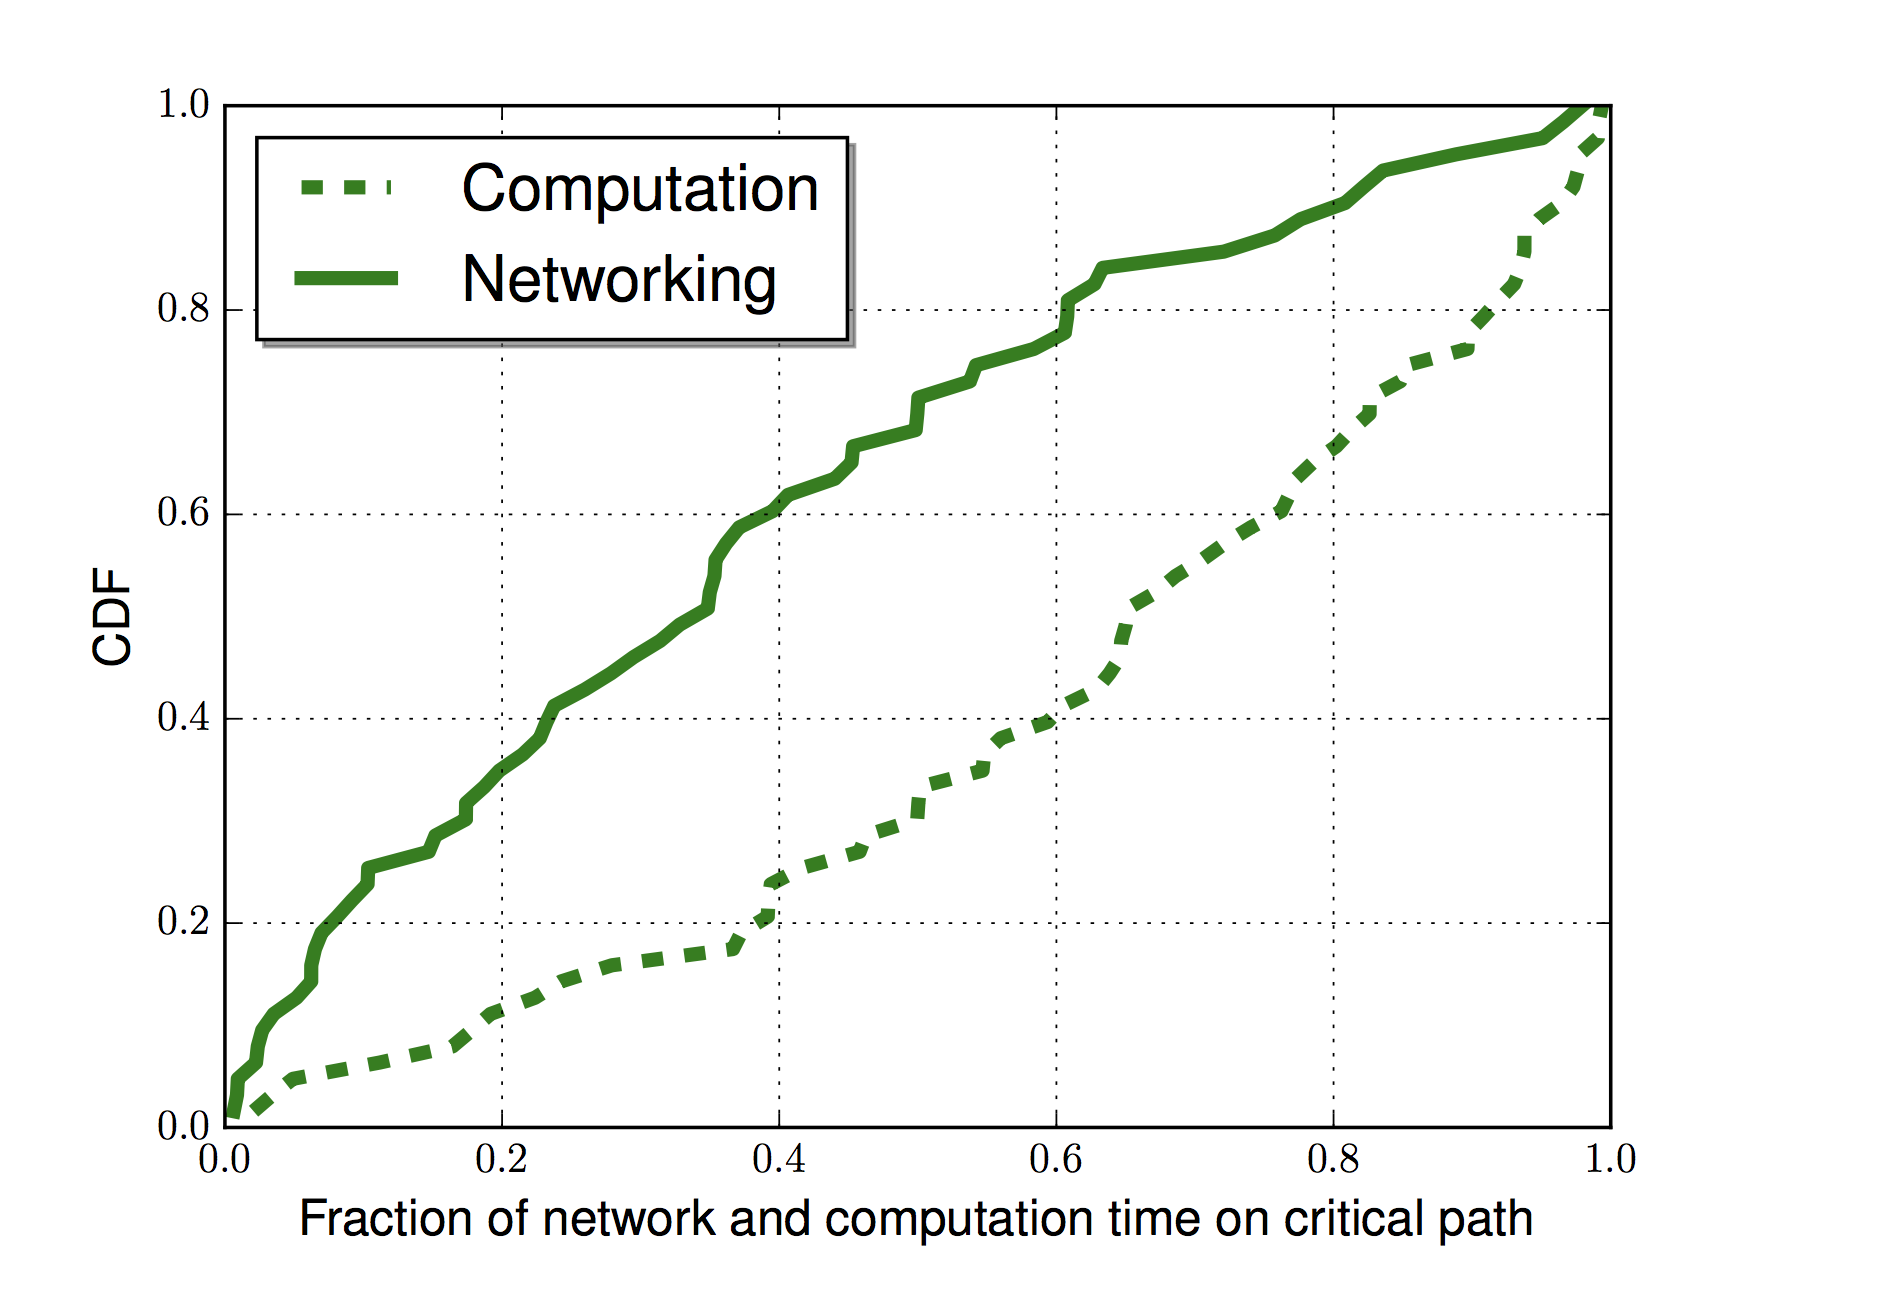
\includegraphics[width=0.9\columnwidth]{figs/comp_net.png}
\tightcaption{Runtime information on mobile devices}
\label{fig:mobile-runtime}
\end{figure}

\begin{figure}[t]
\centering
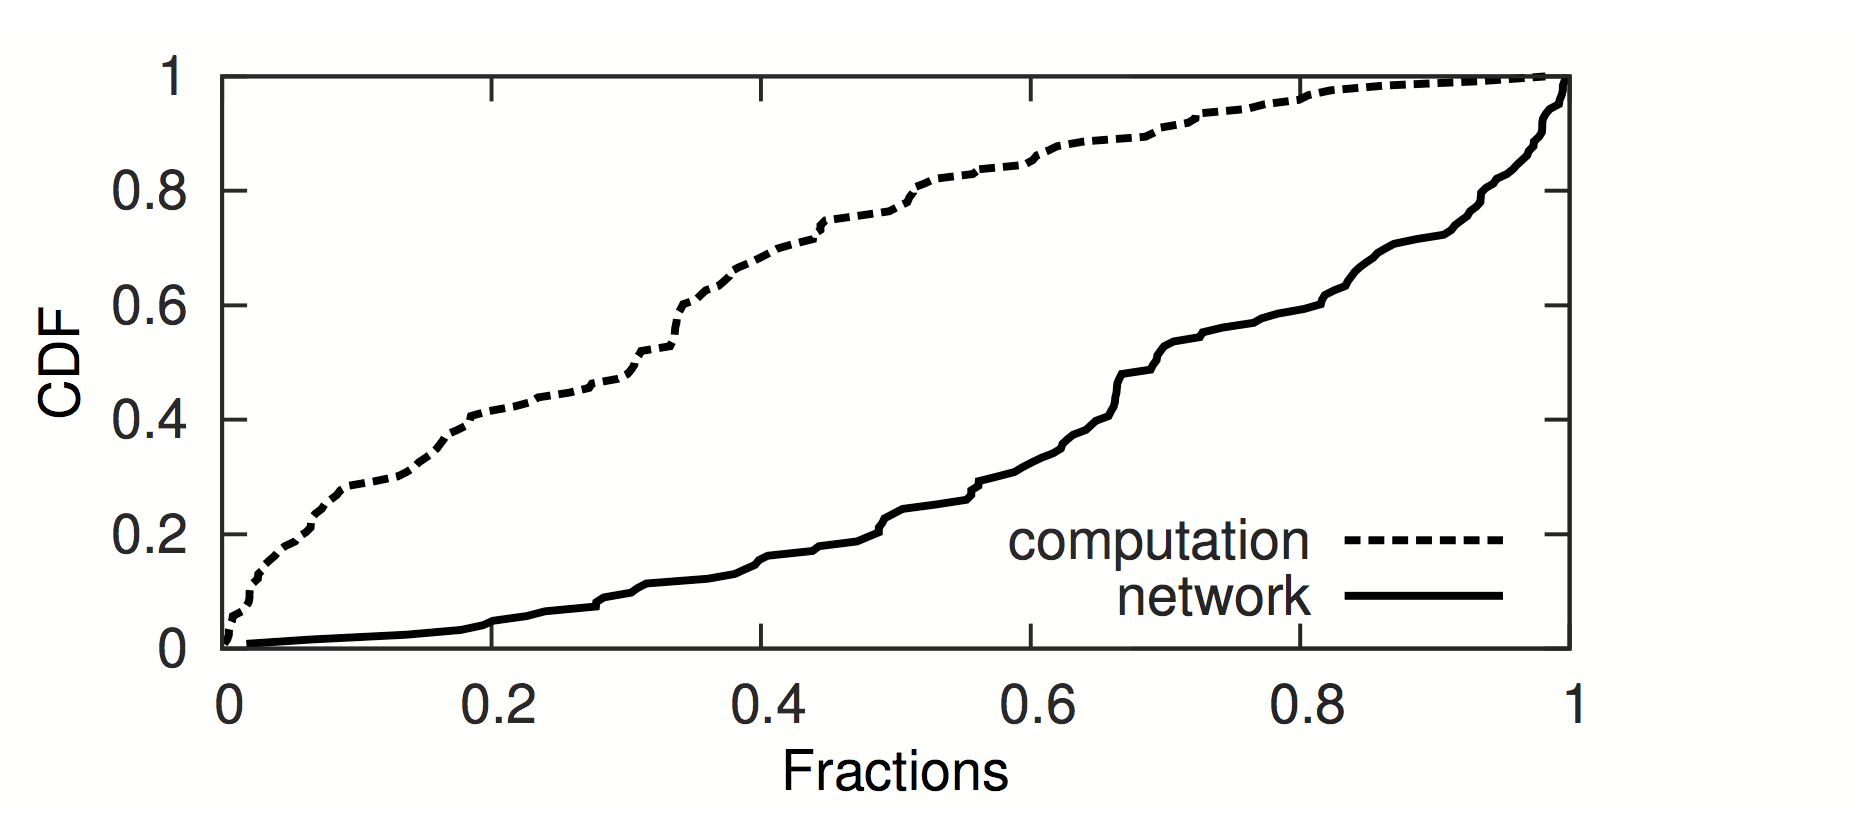
\includegraphics[width=0.9\columnwidth]{figs/comp_net_desk.png}
\tightcaption{Runtime information on desktops}
\label{fig:mobile-runtime}
\end{figure}

% \begin{figure}[t]
% \centering
% \begin{tabular}{cc}
% 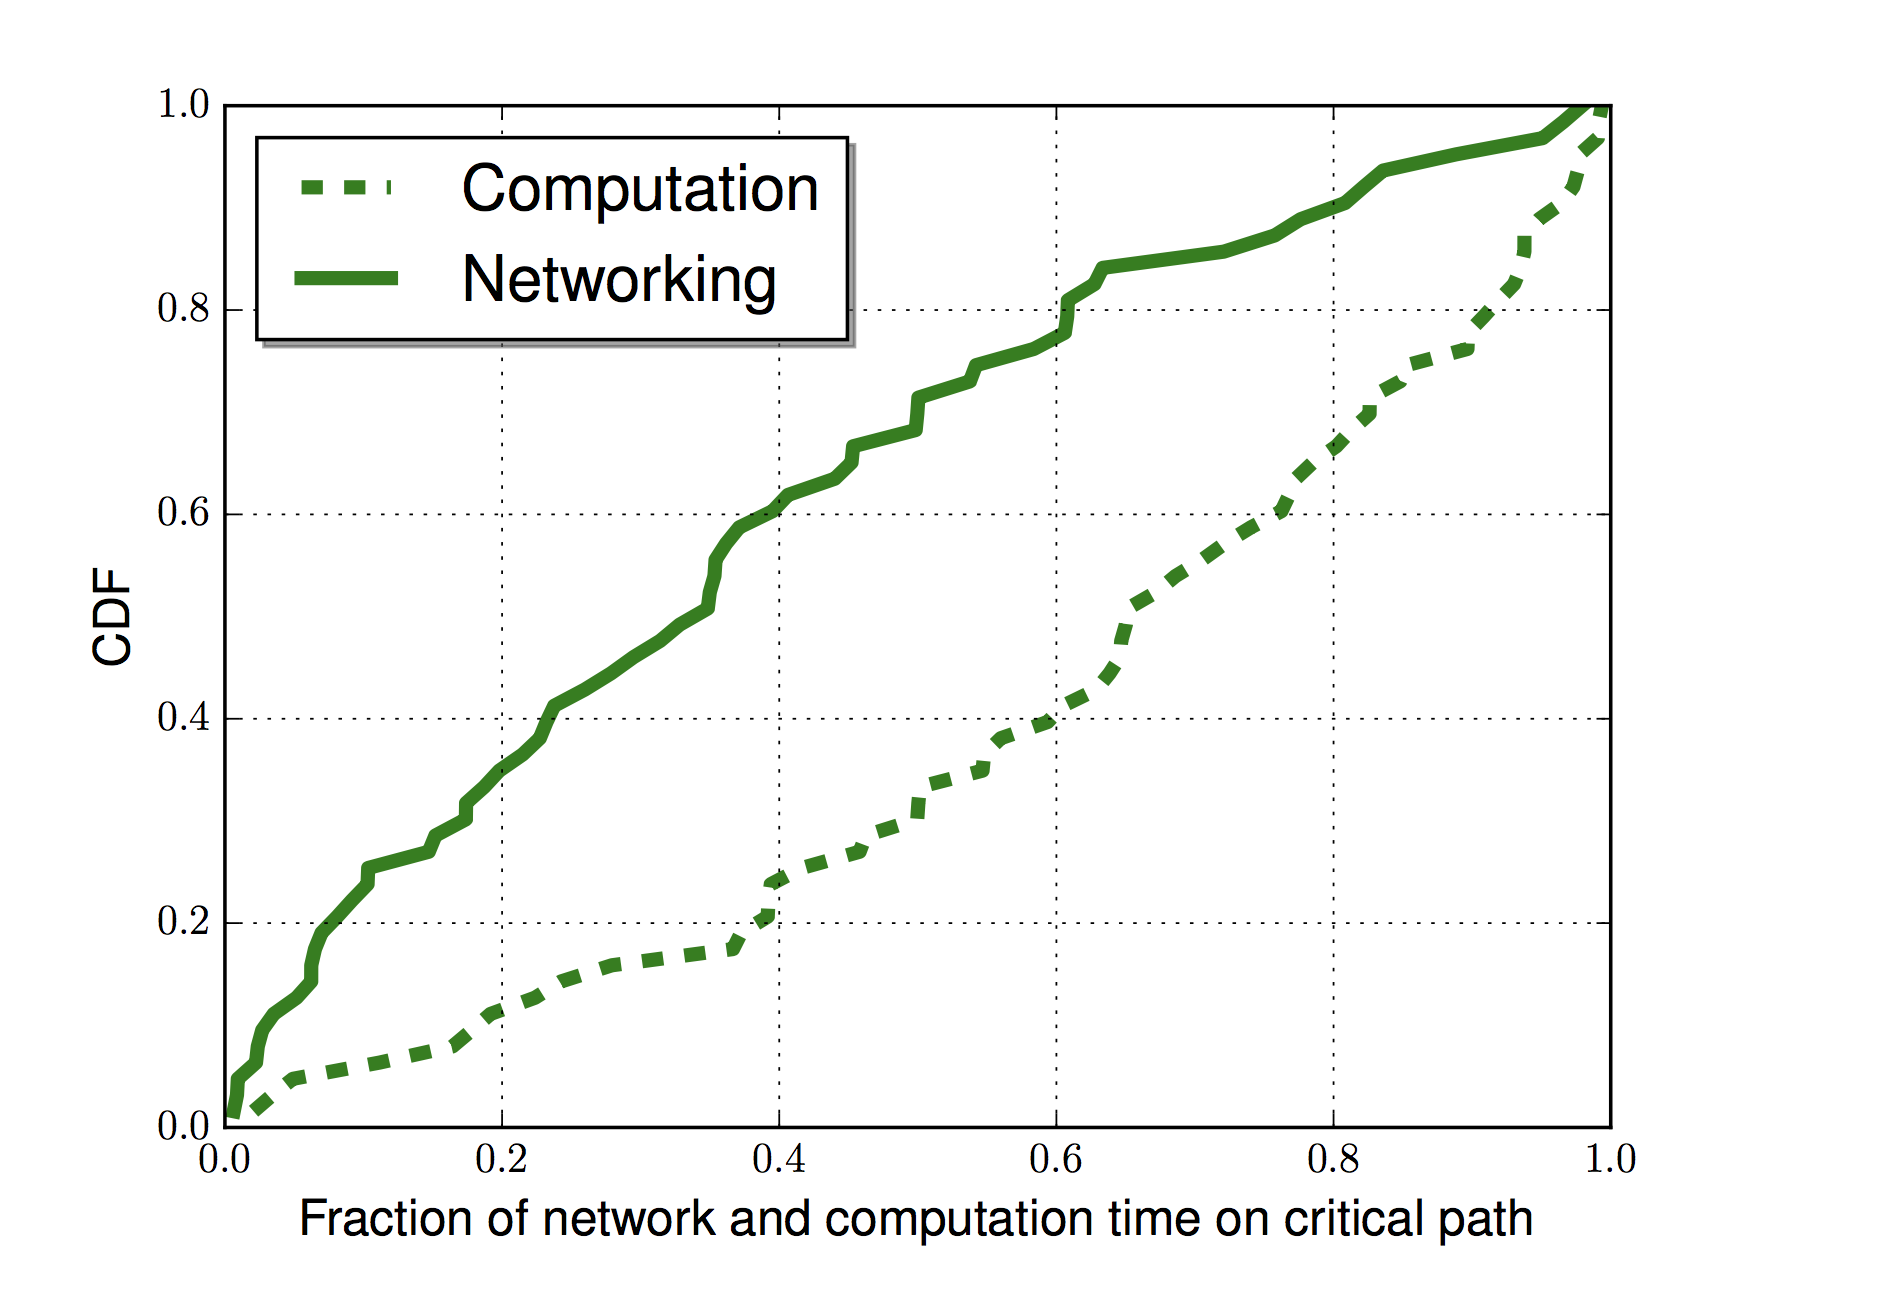
\includegraphics[width=0.9\columnwidth]{figs/comp_net.png}&
% 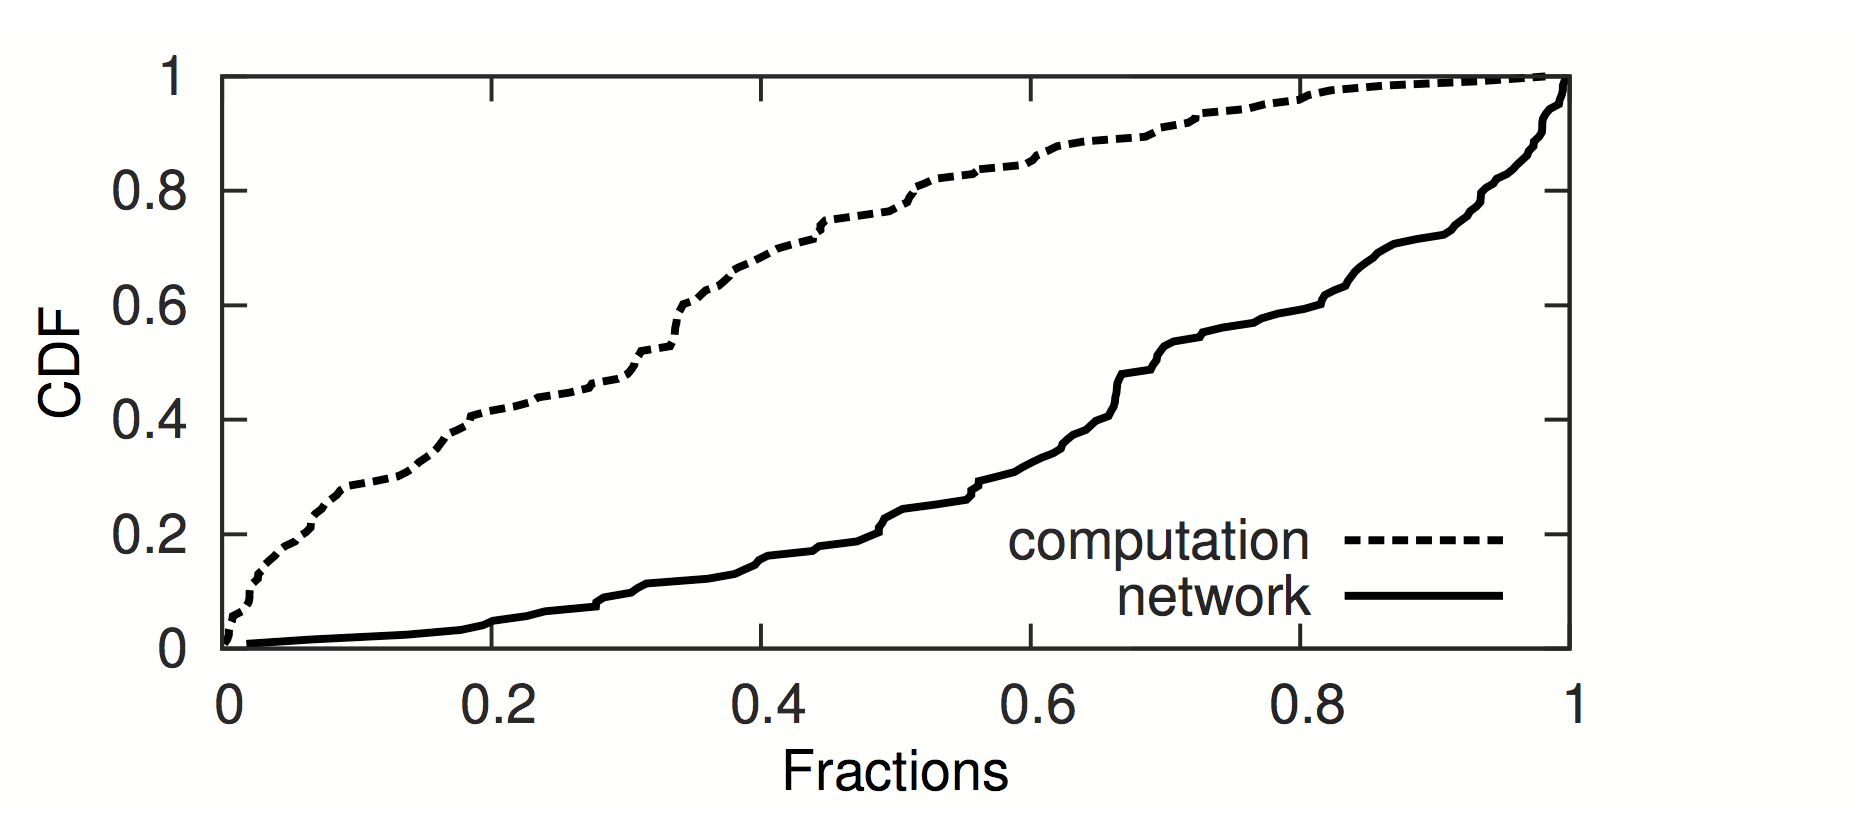
\includegraphics[width=0.9\columnwidth]{figs/comp_net_desk.png}\\
% {\small (a) Azure} & {\small (b) AWS}
% \end{tabular}
% \label{fig:dcs-local}
% \end{figure}

We propose a new technique to improve the page load time by reducing the javscript time. %Which part of the javascript time here? 
In order to do this, we intend to build a new caching framework for the modern web browsers,
specifically Google Chrome. We choose to focus on Chrome because it accounts for about 50\% of the market share in terms of browser
usage. Our caching framework will store the javascript execution result. This can mean a lot of things
due to the dynamic nature javascript. Most of the times it is simply the return value of the 
javascript functions. At other times it can be a modified DOM structure or just some intermediate result which
will be further processed by other javascript functions, later down the execution timeline. 
The expiry of this javascript exectution cache is supposed to be same as the expire of the javascript source cache. % I don't understand what this sentence means but it may be right?
There are a lot of caveats to this approach, and in our work we will explore all of these. % Again, this is really vague and I don't really understand what this means...
The biggest challenge when developing a new caching framework is modifying the current browser's code 
in order to evaluate the efficacy of our caching framework. Since a lot of browsers already implement caching
at the javascript runtime level, such as compiler and parser caches, a lot of this architecure can be borrowed
for the execution cache as well. 
Another potential challenge will be the memory overhead. Most of the popular websites which spend about 70\% 
of their time on javascript execution are running 1000s of javascript functions. Saving the output of all 
of these functions will add extra memory overhead to current browsers. 
